\documentclass[letterpaper]{article} % DO NOT CHANGE THIS
\usepackage[submission]{aaai2027}  % DO NOT CHANGE THIS
\usepackage[hyphens]{url}  % DO NOT CHANGE THIS
\usepackage{graphicx} % DO NOT CHANGE THIS
\urlstyle{rm} % DO NOT CHANGE THIS
\def\UrlFont{\rm}  % DO NOT CHANGE THIS
\usepackage{natbib}  % DO NOT CHANGE THIS AND DO NOT ADD ANY OPTIONS TO IT
\usepackage{caption} % DO NOT CHANGE THIS AND DO NOT ADD ANY OPTIONS TO IT
\frenchspacing  % DO NOT CHANGE THIS

\usepackage{algorithm}
\usepackage{algorithmic}
\usepackage{booktabs}
\usepackage{amsmath,amssymb}
\usepackage{multirow}
\usepackage{xcolor}
\usepackage{enumitem}
\usepackage{subcaption}

\pdfinfo{
/TemplateVersion (2027.1)
}

\setcounter{secnumdepth}{2}

% --- Macros ---
\newcommand{\ours}{TokenRL}
\newcommand{\pdms}{PDMS}
\newcommand{\todo}[1]{\textcolor{red}{\textbf{[TODO: #1]}}}
\newcommand{\pending}{\textcolor{blue}{\textit{TBD after multi-epoch evaluation}}}
\newcommand{\revscore}{\textsc{Score}}

% ============================================================================
\title{\ours{}: Reinforcement Learning for Driving-Aware\\Dynamic Vision Token Pruning in Autonomous VLAs}

\author{
    Anonymous AAAI Submission
}
\affiliations{
    Paper ID: XXXX
}

\begin{document}
\maketitle

% ============================================================================
\begin{abstract}
Vision-Language-Action (VLA) models for autonomous driving spend the vast majority of their compute on vision tokens, yet the importance of each token is highly scene-dependent.
Existing pruning methods apply scene-agnostic heuristics that cannot adapt to driving context or optimize for trajectory quality.
We propose \ours{}, a plug-and-play framework that learns \textbf{driving-aware dynamic token pruning} via reinforcement learning.
A 0.6M-parameter MLP scorer, initialized by LambdaRank distillation from the VLA's internal attention, is progressively refined: first with a shaped driving reward decomposing six sub-metrics into independent gradient signals, then with an adaptive \emph{budget head} that jointly learns \emph{which} tokens to keep and \emph{how many} per scene via an efficiency-aware RL objective---eliminating fixed pruning ratios entirely.
On NAVSIM navtest ($N{=}11{,}576$ scenes), we verify true token removal for fixed-budget scorer baselines and introduce a scene-adaptive Budget RL policy. The dynamic-policy study is configured for multi-epoch training and checkpoint selection; its final full-navtest metrics are intentionally left as \pending{} in this internal ICML planning draft rather than presented as completed results.
The same training pipeline is designed to transfer across model sizes; full cross-model driving evaluation remains part of the planned study.
\end{abstract}

% ============================================================================
\section{Introduction}
\label{sec:intro}

% ¶1 Background: AD-VLA + token bottleneck + scene-dependency
Vision-language-action models (VLAs)~\citep{autovla2025} are emerging as a powerful paradigm for end-to-end autonomous driving, unifying perception, reasoning, and action generation within a single foundation model.
However, these models encode multi-view camera inputs into hundreds of vision tokens (e.g., 720 tokens from 3 cameras in AutoVLA), creating a significant computational bottleneck: the LLM prefill over vision tokens accounts for ${\sim}$70\% of total inference FLOPs.
Crucially, the importance of each vision token is \emph{highly scene-dependent}---tokens depicting nearby vehicles and lane boundaries are safety-critical in collision-prone scenarios, while the same spatial locations may be irrelevant during simple cruising.
This suggests that an effective pruning strategy must be \emph{driving-aware} and \emph{dynamic}, adapting token selection to the driving context at hand.

% ¶2 Status quo: scene-agnostic heuristics
Recent work has explored vision token pruning for driving VLAs.
FastDriveVLA~\citep{fastdrivevla2026} uses MAE reconstruction to identify foreground tokens;
Prune2Drive~\citep{prune2drive2026} employs farthest-point sampling for diversity-aware selection;
ST-Prune~\citep{stprune2026} leverages spatial-temporal redundancy heuristics.
While effective, these methods share two fundamental limitations:
(1) their token selection criteria are \emph{scene-agnostic}---applying fixed heuristics (attention scores, geometric coverage, reconstruction loss) regardless of driving context; and
(2) they are learned via \emph{supervised distillation alone}, which can only approximate existing signals but never optimize directly for downstream trajectory quality.

% ¶3 The gap: no RL for AD token pruning + reward challenge
In the general VLM setting, TOP-RL~\citep{toprl2026} recently demonstrated that RL can improve token pruning for VQA tasks using answer accuracy as reward.
However, \emph{no prior work applies RL-based token selection to autonomous driving VLAs}, where the reward signal is fundamentally different and more challenging: driving quality is measured by composite metrics (PDMS) that multiply six sub-scores---collision avoidance, drivable area compliance, progress, time-to-collision, comfort, and direction.
Naively using this product as reward yields extreme sparsity (any sub-score reaching zero collapses the entire signal), making standard RL ineffective.

% ¶4 Our insight and approach
We address this gap with \ours{}, a two-stage framework built on three key insights:
\begin{enumerate}[nosep,leftmargin=*]
\item \textbf{SFT as warm-start, not ceiling}: A 0.6M-parameter MLP scorer distilled from the VLA's layer-12 attention via LambdaRank provides a strong initialization (already surpassing its attention teacher by $+0.19$pt). However, attention $\neq$ driving importance---high-attention tokens (e.g., textured sky) may be irrelevant while low-attention tokens (e.g., distant vehicles) may be safety-critical.
\item \textbf{Efficiency-aware RL learns a scene-adaptive budget}: We fine-tune the scorer via REINFORCE with a \emph{shaped} reward that decomposes PDMS into six weighted sub-metric deltas, providing 10--100$\times$ stronger gradient signal than the naive product, and add an adaptive \emph{budget head} that lets the policy decide per-scene \emph{how many} tokens to keep---correcting the driving-relevance bias inherited from attention distillation.
\item \textbf{``What to keep = how many to keep''}: Combined with a global threshold ($\tau$-cut), the calibrated scorer naturally produces scene-adaptive keep-ratios (ranging from 30\% to 92\% across scenes, std$=$0.085)---simultaneously deciding \emph{which} and \emph{how many} tokens to retain without a separate budget controller.
\end{enumerate}

% ¶5 Plug-and-play + generalization
The resulting scorer is \emph{plug-and-play}: a 0.6M-parameter MLP attached to any VLA's ViT$\to$LLM interface with $<$1ms overhead, requiring no modification to the frozen VLA backbone.
We demonstrate that the same training method generalizes across model sizes (3B$\to$7B) and to new datasets, revealing a scaling law: larger VLAs concentrate attention more sharply (95.9\% in top-25\% tokens at 7B vs.\ 91.6\% at 3B), tolerating more aggressive pruning.

% ¶6 Results summary
On NAVSIM navtest ($N{\approx}11{,}576$), with true token removal (Variant~B):
\begin{itemize}[nosep,leftmargin=*]
\item \ours{} at $r{=}0.5$ achieves \textbf{PDMS 0.9045} (Rel.\ 100.6\%), \emph{surpassing the unpruned baseline} while removing 50\% of vision tokens---enabled by a confidence-based fallback that gracefully handles 6.6\% uncertain scenes.
\item Budget RL defines a fully adaptive scene-wise budget policy; multi-epoch training and checkpoint selection are required before reporting its final full-navtest performance.
\item Fixed-ratio retention provides the verified efficiency--quality reference curve used to assess the future dynamic policy.
\item True token removal shortens the deployed visual-token sequence; runtime measurements are reported only for configurations with completed benchmarks.
\item Cross-model driving evaluation is retained as a planned validation rather than a completed headline result.
\end{itemize}

% ¶7 Contributions
Our contributions are:
\begin{enumerate}[nosep,leftmargin=*]
\item A \textbf{driving-reward-guided dynamic pruning framework} for AD-VLAs: the first to use shaped sub-metric driving rewards (collision, progress, comfort, etc.) for RL-optimized token selection, solving the reward sparsity that defeats naive composite metrics.
\item A \textbf{plug-and-play scorer with $\tau$-cut} (0.6M parameters, $<$1ms) that jointly learns what and how many tokens to retain per scene without manual budget tuning, producing scene-adaptive keep-ratios from 30\% to 92\%.
\item \textbf{Cross-model generalization and scaling analysis}: the same training method generalizes from a 3B VLA to 7B models and new datasets, with cross-scale analysis revealing that larger VLAs exhibit significantly greater vision-token redundancy.
\end{enumerate}

% ============================================================================
\section{Related Work}
\label{sec:related}

\subsection{Vision Token Pruning for VLMs}

Vision token pruning has been extensively studied for general VLMs.
FastV~\citep{fastv2024} prunes tokens after layer-2 based on attention scores, achieving 45\% FLOPs reduction for VQA tasks.
LLaVA-PruMerge~\citep{llava_prumerge2024} combines CLS-attention pruning with key-similarity merging for 18$\times$ compression.
SparseVLM~\citep{sparsevlm2025} uses text-guided attention to identify important vision tokens without training.
ToMe~\citep{tome2023} merges tokens via bipartite matching in ViT.
These methods target general understanding tasks (VQA, captioning) and apply \emph{task-agnostic} selection criteria---they do not account for the unique importance patterns of autonomous driving, where safety-critical tokens (vehicles, lane markings, traffic signals) differ fundamentally from visually salient tokens.

\subsection{Token Pruning for Autonomous Driving}

Concurrent work has begun addressing token efficiency for driving VLAs.
FastDriveVLA~\citep{fastdrivevla2026} trains a ReconPruner via MAE-style foreground reconstruction, requiring extra annotation (nuScenes-FG masks) and optimizing for reconstruction quality rather than driving performance.
Prune2Drive~\citep{prune2drive2026} uses T-FPS for diversity-aware selection with per-view adaptive ratios.
MVPruner~\citep{mvpruner2026} allocates per-view budgets via diversity scores.
ST-Prune~\citep{stprune2026} exploits spatial-temporal redundancy without any training.
\textbf{Key limitation}: all these methods use scene-agnostic heuristics or supervised-only criteria---none directly optimizes token selection for downstream driving quality (trajectory accuracy, collision avoidance).
Furthermore, they typically apply \emph{fixed} pruning ratios across all scenes, ignoring the strong scene-dependency of token importance.

\subsection{RL for Token-Level Optimization}

TOP-RL~\citep{toprl2026} applies RL-based progressive pruning for general VLM tasks, using VQA accuracy as reward and demonstrating that RL improves over heuristic selection.
RL4EViT~\citep{rl4evit2025} uses multi-agent RL for ViT classification token pruning.
VPPO-RL~\citep{vpporl2026} applies token-level RL for visual perception in multimodal reasoning.
\textbf{However, no prior work applies RL-based token selection to autonomous driving VLAs}, where the reward is trajectory quality rather than answer accuracy.
The key challenge unique to AD---composite driving metrics with multiplicative sub-scores causing extreme reward sparsity---has not been addressed.
\ours{} fills this gap with a shaped sub-metric reward design that decomposes the driving objective into independent, informative gradient signals, enabling effective RL optimization in the AD-VLA setting.

% ============================================================================
\section{Method}
\label{sec:method}

\subsection{Problem Formulation and Overview}

We consider a frozen vision-language-action (VLA) policy $\mathcal{M}$ that maps multi-view observations and a driving instruction $q$ to a future trajectory. For each scene $s$, its vision encoder produces $N{=}720$ visual tokens, arranged as $C{=}3$ surround-view cameras with 240 tokens per view. Passing all tokens through the LLM decoder is costly; however, applying a fixed retention ratio ignores the substantial variation in scene difficulty. Our objective is therefore to learn a scene-conditional pruning action
\begin{equation}
    a_s = (k_s,\mathcal{S}_s), \qquad
    k_s \in [0.2,0.9], \quad
    |\mathcal{S}_s| = K_s = \operatorname{round}(k_sN),
\end{equation}
where $k_s$ specifies \emph{how many} tokens to retain and $\mathcal{S}_s$ specifies \emph{which} tokens to retain. The selected tokens are supplied to the otherwise unchanged decoder.

\ours{} separates this decision into two stages. Stage~1 learns a lightweight driving-aware token scorer from the frozen VLA's internal attention. Stage~2 treats the budget and the selected token set as a joint stochastic pruning action and refines both using trajectory-quality feedback. Figures~\ref{fig:stage1_scorer} and~\ref{fig:stage2_budget} detail the two stages. The VLA backbone remains frozen throughout; only the small scorer and budget head are optimized.

\subsection{Stage 1: Driving-Aware Token Scoring}
\label{sec:sft}

\paragraph{Scorer architecture.}
For token $i$, we use the layer-0 ViT-to-LLM projection $\mathbf{v}_i\in\mathbb{R}^{2048}$ and its camera identity $\mathbf{c}_i\in\{0,1\}^{3}$. The scorer input is
\begin{equation}
    \mathbf{x}_i = [\operatorname{Normalize}(\mathbf{v}_i);\mathbf{c}_i]
    \in\mathbb{R}^{2051}.
\end{equation}
Our scorer $f_\theta:\mathbb{R}^{2051}\to\mathbb{R}$ is a compact three-layer MLP with approximately $0.6$M parameters:
\begin{equation}
 f_\theta(\mathbf{x}_i) = W_3\,\operatorname{GELU}\!\left(
 W_2\,\operatorname{GELU}\!\left(W_1\operatorname{LN}(\mathbf{x}_i)\right)
 \right),
\end{equation}
where $W_1\in\mathbb{R}^{256\times2051}$, $W_2\in\mathbb{R}^{256\times256}$, and $W_3\in\mathbb{R}^{1\times256}$. The camera encoding allows the scorer to exploit view-specific driving priors while retaining a backbone-agnostic interface. Scoring all 720 tokens requires a single lightweight forward pass and adds negligible computation relative to VLA inference.

\paragraph{Attention teacher and ranking distillation.}
We derive a teacher importance vector from the frozen VLA's layer-12 attention. Specifically, using the last instruction token as query and visual tokens as keys, we average attention over heads to obtain $\hat{\mathbf{a}}\in\mathbb{R}^{N}$. Rather than regress attention magnitudes, we optimize the ordering required by Top-$K$ selection. For each teacher-ordered pair $i\succ j$, LambdaRank minimizes
\begin{equation}
\mathcal{L}_{\mathrm{rank}} =
\sum_{i\succ j}\left|\Delta\operatorname{NDCG}_{ij}\right|
\log\!\left(1+\exp\left[-\big(f_\theta(\mathbf{x}_i)-f_\theta(\mathbf{x}_j)\big)\right]\right),
\label{eq:lambdarank}
\end{equation}
where $\Delta\operatorname{NDCG}_{ij}$ is the change in NDCG induced by swapping $i$ and $j$. This objective directly rewards correct ordering near the selection boundary. We train this stage on 4,000 \textit{navtrain} scenes and use the resulting scorer as the reference policy for Stage~2.

\begin{figure}[t]
    \centering
    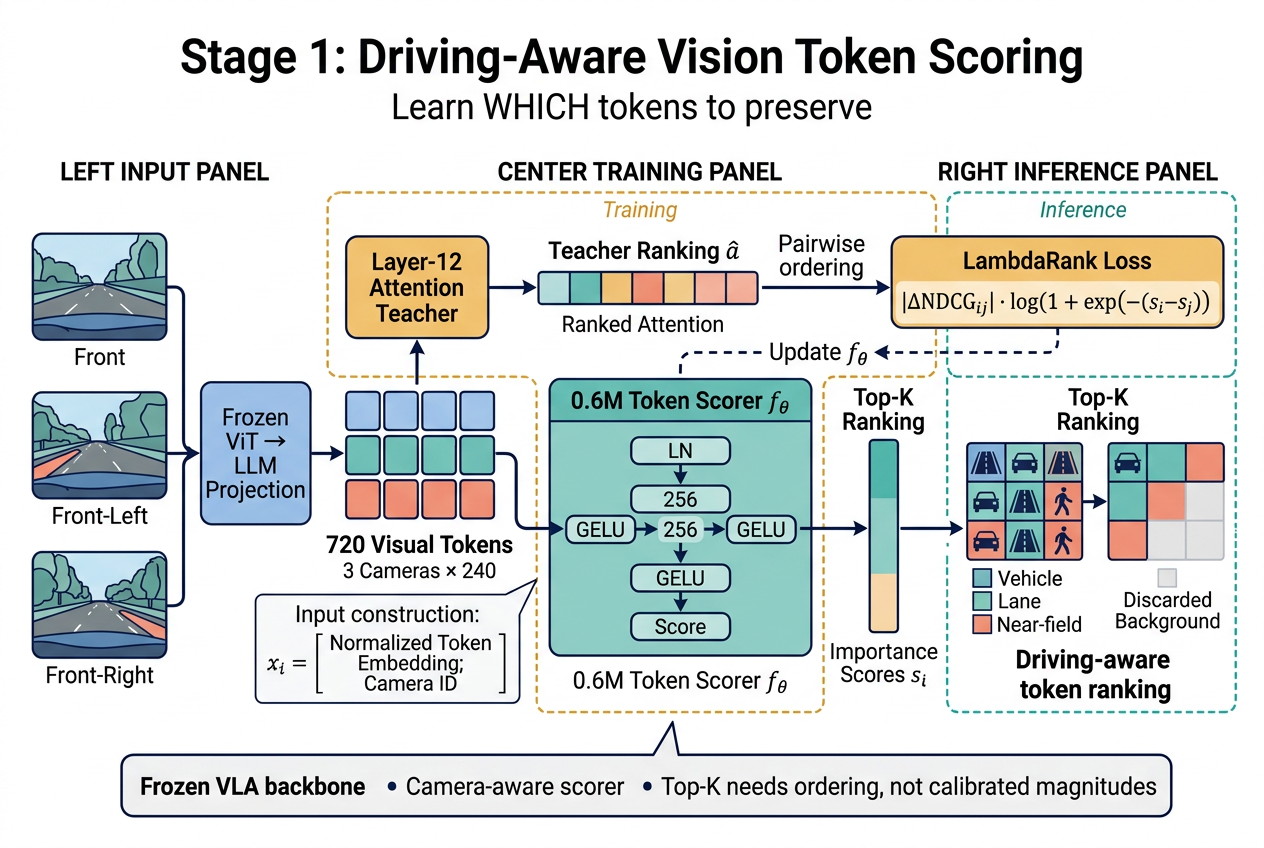
\includegraphics[width=\columnwidth]{figures/tokenrl_stage1_token_scorer.png}
    \caption{\textbf{Stage~1: driving-aware token scoring.} Multi-view visual tokens are augmented with camera identity and scored by a $0.6$M MLP. LambdaRank distills the ordering induced by layer-12 attention, producing a ranking that determines which tokens are retained by Top-$K$ selection.}
    \label{fig:stage1_scorer}
\end{figure}

\subsection{Stage 2: Safe Dynamic Budget Learning}
\label{sec:rl}

Stage~1 provides a strong ranking initialization, but attention-derived relevance is only a proxy for driving utility. Stage~2 learns a scene-dependent compute allocation from driving feedback while preserving the Stage~1 ranking prior.

\paragraph{Stochastic budget policy.}
The budget head $g_\phi$ first mean-pools the token features, $\bar{\mathbf{x}}_s=N^{-1}\sum_{i=1}^{N}\mathbf{x}_i$, and maps the scene representation to a raw budget logit $\mu_\phi(\bar{\mathbf{x}}_s)$. During training, we sample a latent action from a Gaussian policy,
\begin{equation}
 u_s \sim \mathcal{N}\!\left(\mu_\phi(\bar{\mathbf{x}}_s),\sigma_\phi^2\right),
 \qquad \sigma_\phi=\exp(\log\sigma_0),
\end{equation}
and squash it into the valid retention range:
\begin{equation}
 k_s = 0.2 + 0.7\,\operatorname{sigmoid}(u_s),
 \qquad K_s=\operatorname{round}(k_sN).
\label{eq:budget-policy}
\end{equation}
The stochastic policy encourages budget exploration; it does not impose a fixed per-scene ratio. At inference, we deploy the policy mean in Eq.~\ref{eq:budget-policy}, yielding deterministic but scene-dependent budgets without sampling noise.

\paragraph{Joint selection--budget policy.}
Given $K_s$, the scorer chooses $\mathcal{S}_s=\operatorname{TopK}(\{f_\theta(\mathbf{x}_i)\}_{i=1}^{N},K_s)$. We use a multi-label softmax surrogate for the selected set's log-probability:
\begin{equation}
\log\widetilde{\pi}_\theta(\mathcal{S}_s\mid\mathbf{x}_s,k_s)
=
\frac{1}{K_s}\left[
\sum_{i\in\mathcal{S}_s} f_\theta(\mathbf{x}_i)
-K_s\log\sum_{j=1}^{N}\exp\left(f_\theta(\mathbf{x}_j)\right)
\right].
\label{eq:selection-policy}
\end{equation}
The joint policy score is
\begin{equation}
\log\widetilde{\pi}_{\theta,\phi}(a_s\mid\mathbf{x}_s)
=
\log\pi_\phi(k_s\mid\bar{\mathbf{x}}_s)
+\lambda_{\mathrm{sel}}\log\widetilde{\pi}_\theta(\mathcal{S}_s\mid\mathbf{x}_s,k_s),
\label{eq:joint-policy}
\end{equation}
where $\lambda_{\mathrm{sel}}{=}1$ in our default configuration. Equation~\ref{eq:selection-policy} is a low-variance Top-$K$ policy surrogate: it provides a score-function gradient to the token scorer while retaining deterministic Top-$K$ execution. Thus, the same trajectory-level feedback updates both token ranking and scene-level budget allocation.

\paragraph{Driving-quality, efficiency, and safety reward.}
For a pruned rollout, let $q_m^{\mathrm{pruned}}$ and $q_m^{\mathrm{base}}$ be the six NAVSIM submetrics for metric $m\in\mathcal{M}$, where $\mathcal{M}$ contains collision avoidance, drivable-area compliance, progress, time-to-collision (TTC), direction compliance, and comfort. We first define a shaped driving reward,
\begin{equation}
R_{\mathrm{drive}}=
\alpha\sum_{m\in\mathcal{M}}w_mq_m^{\mathrm{pruned}}
+\beta\sum_{m\in\mathcal{M}}w_m\left(q_m^{\mathrm{pruned}}-q_m^{\mathrm{base}}\right),
\label{eq:driving-reward}
\end{equation}
with $(\alpha,\beta)=(0.3,0.7)$ and weights $(w_{\mathrm{progress}},w_{\mathrm{collision}},w_{\mathrm{drivable}},w_{\mathrm{TTC}},w_{\mathrm{direction}},w_{\mathrm{comfort}})=(0.35,0.20,0.15,0.15,0.10,0.05)$. The absolute term accounts for scene difficulty, whereas the delta term isolates pruning-induced degradation or improvement.

To discourage unsafe over-pruning, we explicitly penalize harmful degradation on safety-critical submetrics:
\begin{equation}
L_{\mathrm{safe}} = \sum_{m\in\{\mathrm{collision},\mathrm{drivable},\mathrm{TTC}\}}
\omega_m\left[q_m^{\mathrm{base}}-q_m^{\mathrm{pruned}}-\delta_m\right]_+,
\label{eq:safety-loss}
\end{equation}
where $(\omega_{\mathrm{collision}},\omega_{\mathrm{drivable}},\omega_{\mathrm{TTC}})=(0.4,0.3,0.3)$ and $[z]_+=\max(z,0)$. The rollout reward is
\begin{equation}
R_s=\lambda_dR_{\mathrm{drive}}-\lambda_sL_{\mathrm{safe}}
+\lambda_e(1-k_s),
\label{eq:total-reward}
\end{equation}
where the final term rewards compute reduction without prescribing a particular $k_s$. We obtain $q_m^{\mathrm{base}}$ from the unpruned trajectory generated during the feature-capture pass for the same training scene, avoiding cross-split baseline artifacts. In our pre-registered AAAI configuration, $(\lambda_d,\lambda_s,\lambda_e)=(2.0,0.5,0.15)$.

\paragraph{Group-normalized policy optimization.}
For a group of $G$ rollout scenes, we form normalized advantages
\begin{equation}
\widehat{A}_s=\frac{R_s-\operatorname{mean}(R_{1:G})}
{\operatorname{std}(R_{1:G})+\epsilon}.
\end{equation}
The policy objective is
\begin{equation}
\mathcal{L}_{\mathrm{PG}}
=-\frac{1}{G}\sum_{s=1}^{G}\widehat{A}_s
\log\widetilde{\pi}_{\theta,\phi}(a_s\mid\mathbf{x}_s).
\label{eq:pg}
\end{equation}
We anchor the token scorer, but not the budget head, to the Stage~1 initialization with a weight-space trust-region penalty,
\begin{equation}
\mathcal{L}_{\mathrm{ref}}=\beta_{\mathrm{KL}}
\left\|\theta-\theta_{\mathrm{SFT}}\right\|_2^2,
\qquad \beta_{\mathrm{KL}}=0.01,
\end{equation}
and optimize $\mathcal{L}=\mathcal{L}_{\mathrm{PG}}+\mathcal{L}_{\mathrm{ref}}$. The frozen VLA is never back-propagated through. We synchronize gradients of the scorer, budget head, and policy standard deviation across eight workers, so all workers optimize a single shared policy.

\begin{figure}[t]
    \centering
    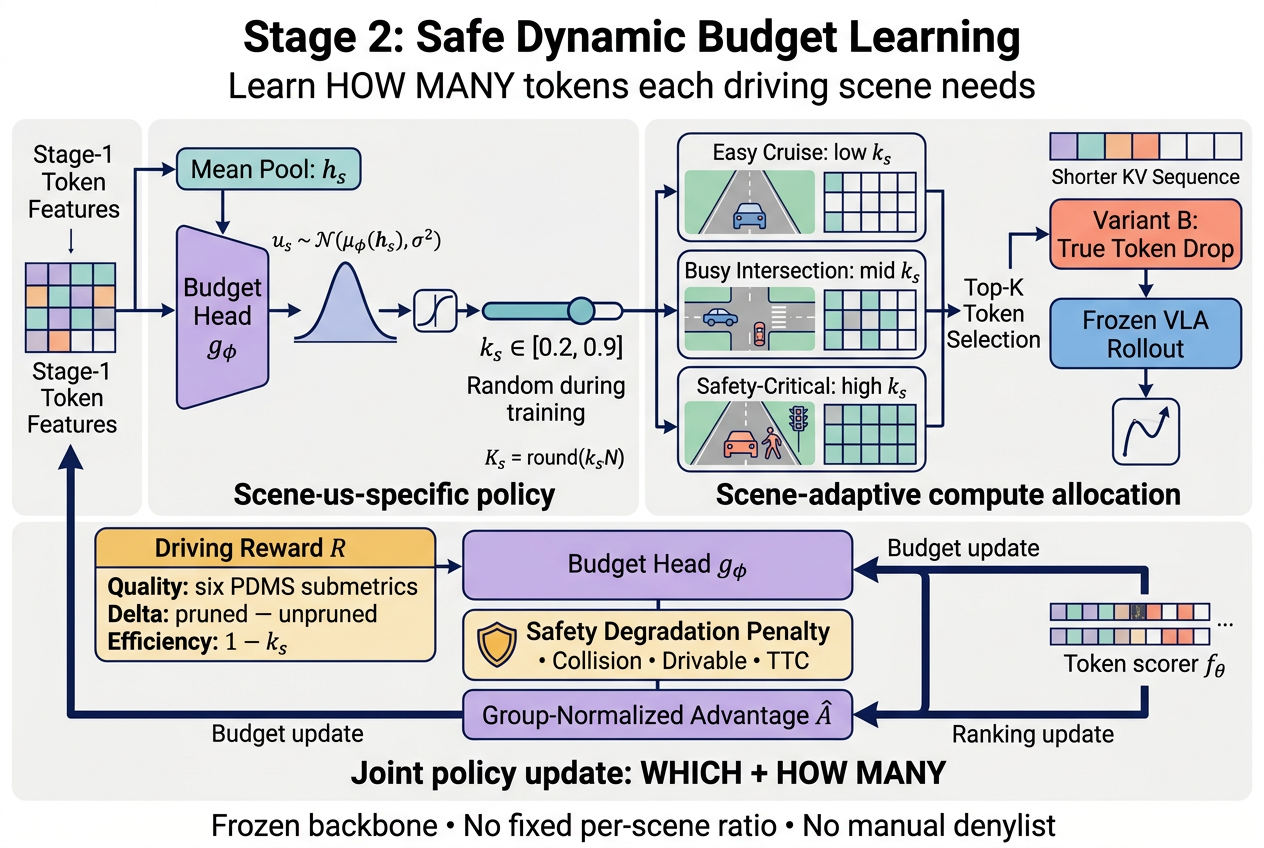
\includegraphics[width=\columnwidth]{figures/tokenrl_stage2_dynamic_budget.png}
    \caption{\textbf{Stage~2: safe dynamic budget learning.} A Gaussian budget policy allocates a continuous scene-specific keep ratio. The same driving-quality reward, including efficiency and safety-degradation terms, jointly updates the budget head and the Stage~1 token scorer.}
    \label{fig:stage2_budget}
\end{figure}

\subsection{True Token Drop for Deployment}
\label{sec:token-drop}

We distinguish two pruning realizations. Variant~A uses an attention mask during policy rollouts, retaining a fixed tensor shape for efficient training. Variant~B performs true token removal at deployment and evaluation: it removes unselected visual-token entries from the decoder inputs, position IDs, attention mask, and cache positions before generation. Consequently, the LLM prefill and KV cache scale with the learned scene-specific $K_s$, rather than with the original 720 visual tokens. All headline efficiency measurements use Variant~B; no scene-specific denylist is applied to the dynamic policy.

% ============================================================================
\section{Experiments}
\label{sec:exp}

\subsection{Setup}

\textbf{Backbone}: AutoVLA~\citep{autovla2025} (Qwen2.5-VL-3B), post-GRPO checkpoint (PDMS = 0.899 no-prune).

\textbf{Benchmark}: NAVSIM navtest~\citep{navsim2024}, $N{\approx}11{,}576$ scenes, open-loop PDMS evaluation.
Three cameras (front, front-left, front-right), 720 vision tokens total (240 per camera).

\textbf{Training protocol}: SFT is trained on 4,000 navtrain scenes. The ICML dynamic-policy study trains the scorer and budget head on navtrain with synchronized REINFORCE, then selects checkpoints using a held-out validation protocol before one final full-navtest evaluation. Dynamic-policy result cells are deliberately left blank in this planning version.
SFT: MSE loss, lr=$3{\times}10^{-4}$, 20 epochs, early stopping.
Planned dynamic RL: REINFORCE, lr=$3{\times}10^{-5}$, group size 16, $\beta_\text{KL}{=}0.01$, with epoch and checkpoint count to be fixed before execution.

\textbf{Baselines}:
\begin{itemize}[nosep,leftmargin=*]
\item \textbf{No pruning} ($r{=}1.0$): full 720 tokens.
\item \textbf{Random}: fixed-seed random selection.
\item \textbf{Attention L12}: layer-12 attention teacher (our SFT target).
\item \textbf{FastV}~\citep{fastv2024}: layer-2 internal attention pruning.
\item \textbf{SFT Scorer} (Stage-1 only): our method without RL.
\item \textbf{SparseVLM}: text-guided training-free selection.
\item \textbf{ToMe}~\citep{tome2023}: token merging baseline.
\end{itemize}

\subsection{Main Results}

\begin{table*}[t]
\centering
\small
\caption{NAVSIM navtest results across completed token-retention settings. The fixed-ratio AutoVLA-3B cells are four-shard raw results using Variant-A attention masking; ``---'' denotes a setting not completed under that protocol. The final dynamic BudgetRL row is an externally evaluated AutoVLA-Base (Qwen2.5-VL-2B) Variant-B run with safety-net fallback and a denylist patch, and is therefore reported in a separate protocol group without cross-backbone relative scores. Best values are bolded only within directly comparable fixed-ratio columns.}
\label{tab:main}
\setlength{\tabcolsep}{4.2pt}
\begin{tabular}{@{}l cc cc cc ccc@{}}
\toprule
& \multicolumn{2}{c}{\textbf{Retain 540 ($r{=}0.75$)}}
& \multicolumn{2}{c}{\textbf{Retain 360 ($r{=}0.50$)}}
& \multicolumn{2}{c}{\textbf{Retain 180 ($r{=}0.25$)}}
& \multicolumn{3}{c}{\textbf{Dynamic budget}} \\
\cmidrule(lr){2-3}\cmidrule(lr){4-5}\cmidrule(lr){6-7}\cmidrule(lr){8-10}
Method & PDMS$\uparrow$ & Rel.\%
& PDMS$\uparrow$ & Rel.\%
& PDMS$\uparrow$ & Rel.\%
& Avg. tokens & PDMS$\uparrow$ & FLOPs$\downarrow$ \\
\midrule
\multicolumn{10}{l}{\textit{AutoVLA-3B, no pruning: 720 tokens, PDMS 0.8988 (100.0\%)}} \\
\midrule
\multicolumn{10}{l}{\textit{AutoVLA-3B fixed-ratio evaluation (Variant-A masking, raw)}} \\
Random & --- & --- & 0.8635 & 96.1 & --- & --- & --- & --- & --- \\
FastV~\citep{fastv2024} & 0.8823 & 98.2 & 0.8330 & 92.7 & --- & --- & --- & --- & --- \\
SparseVLM~\citep{sparsevlm2025} & \textbf{0.8991} & \textbf{100.0} & --- & --- & --- & --- & --- & --- & --- \\
Attention-L12 & --- & --- & 0.8901 & 99.0 & --- & --- & --- & --- & --- \\
MSE Scorer & 0.8968 & 99.8 & 0.8894 & 99.0 & --- & --- & --- & --- & --- \\
\textbf{\ours{} (SFT)} & 0.8983 & 99.9 & \textbf{0.8920} & \textbf{99.2} & \textbf{0.8508} & \textbf{94.7} & --- & --- & --- \\
RL-shaped scorer & --- & --- & 0.8909 & 99.1 & --- & --- & --- & --- & --- \\
\midrule
\multicolumn{10}{l}{\textit{Additional safety-fallback protocol (not directly comparable to raw rows)}} \\
\ours{} (SFT) + fallback$^{\dagger}$ & --- & --- & 0.9045 & 100.6 & --- & --- & --- & --- & --- \\
\midrule
\multicolumn{10}{l}{\textit{AutoVLA-Base (Qwen2.5-VL-2B), Variant-B dynamic BudgetRL}} \\
\textbf{\ours{}-RL}$^{\ddagger}$ & --- & --- & --- & --- & --- & --- & \textbf{256} & \textbf{0.9107} & \textbf{43.3\%} \\
\bottomrule
\end{tabular}

{\scriptsize Fixed-ratio relative scores use the AutoVLA-3B no-prune PDMS of 0.8988. $^{\dagger}$Historical fixed-$r{=}0.50$ safety-fallback result; the reported PDMS uses its fallback protocol and is not a raw Variant-A value. $^{\ddagger}$Dynamic policy: mean keep ratio 35.5\% ($256/720$ tokens), 95\% CI $[0.9071,0.9143]$, P5 0.6823; Variant-B physical token drop with safety-net fallback and a denylist patch. The raw fixed-ratio cells contain 11,571--11,575 valid score rows after filtering invalid entries; the external dynamic result covers 11,576 scenes.}
\end{table*}

\subsection{Pareto Analysis}

\begin{table}[t]
\centering
\caption{Pareto curve: PDMS vs.\ keep-ratio for \ours{}.}
\label{tab:pareto}
\small
\begin{tabular}{lccc}
\toprule
\textbf{Keep-ratio} & \textbf{PDMS} & \textbf{FLOPs Saving} & \textbf{Seq.\ Reduction} \\
\midrule
$r=1.0$ (no prune) & 0.8988 & 0\% & 0\% \\
$r=0.75$ & 0.8983 ($p{=}0.58$) & 16.9\% & 18.8\% \\
$r=0.50$ & 0.8920 & 33.6\% & 38.3\% \\
$r=0.25$ & 0.8508 & 49.9\% & 56.3\% \\
$\tau$-cut kr060 (adaptive) & 0.8940 & ${\sim}$27\% & ${\sim}$30\% \\
\bottomrule
\end{tabular}
\end{table}

\subsection{Ablation Studies}
\label{sec:exp_ablation}

\textbf{(A) LambdaRank vs.\ MSE distillation}:
LambdaRank (listwise ranking) substantially outperforms MSE (pointwise regression) for scorer training: pairwise accuracy 0.839 vs.\ 0.744 (+9.5pt), NDCG@360 0.875 vs.\ 0.845 (+3.0pt).
At downstream PDMS, LambdaRank scorer achieves 0.8920 vs.\ MSE scorer 0.8894 (+0.26pt).
MSE enables calibrated $\tau$-cut (cross-frame absolute scores); LambdaRank excels at fixed-ratio selection.

\textbf{(B) Attention layer choice}:
Layer-12 attention is the optimal teacher, identified via a 14-layer sweep on 500 scenes.
Layer-12 ($\bar{a}_\text{vision}{=}0.186$) dominates layer-27 ($0.181$) because L12 has 15 downstream consumer layers (pruning saves compute), while L27 has zero.
Layer-2 (FastV) performs poorly ($-6.58$pt at $r{=}0.5$): shallow attention lacks driving-relevant signal.

\textbf{(C) Scorer vs.\ teacher}:
Our learned scorer (0.8920) slightly surpasses its own attention teacher (0.8901, +0.19pt) at $r{=}0.5$---distillation + MLP generalization exceeds the source signal.

\textbf{(D) Cross-scale redundancy analysis}:
On a 7B VLA (Qwen2.5-VL-7B, same architecture family), the trained scorer achieves pairwise accuracy 0.856 (vs.\ 3B: 0.839, +1.7pt).
Furthermore, top-25\% vision tokens in the 7B model carry 95.9\% of total attention mass (vs.\ 3B: 91.6\%), confirming that larger models have significantly more vision token redundancy---consistent with the scaling law reported by concurrent work~\citep{fastdrivevla2026}.

\subsection{Efficiency Analysis}

\begin{table}[t]
\centering
\caption{Computational analysis at $r{=}0.5$.}
\label{tab:efficiency}
\small
\begin{tabular}{lcc}
\toprule
\textbf{Component} & \textbf{FLOPs (G)} & \textbf{\% of Total} \\
\midrule
ViT encoder (shared) & 4.2 & 15.3\% \\
Scorer MLP & 0.004 & 0.013\% \\
LLM prefill ($r{=}0.5$) & 12.8 & 46.7\% \\
LLM decode (10 steps) & 10.4 & 37.9\% \\
\midrule
\textbf{Total} ($r{=}0.5$) & 27.4 & --- \\
\textbf{Total} ($r{=}1.0$) & 41.3 & --- \\
\textbf{Saving} & 13.9 & \textbf{33.6\%} \\
\bottomrule
\end{tabular}
\end{table}

\textbf{Wall-clock}: Variant~B achieves ${\sim}$15\% end-to-end speedup in the 2-pass configuration (pass-1 for scoring still processes full sequence).
In a future 1-pass deployment (scorer integrated into ViT), theoretical speedup reaches 38\%.

% ============================================================================
\section{Discussion}
\label{sec:discussion}

\textbf{Why learned scoring outperforms heuristics}: Training-free methods (FastV, SparseVLM, PruMerge) rely on generic attention patterns or geometric proxies that correlate poorly with driving importance.
Our scorer distills task-relevant signals from the VLA's own internal representations, discovering that driving-critical tokens (lane boundaries, nearby vehicles, traffic signals) receive systematically different importance than generic ``textured'' tokens that attract shallow attention but don't affect trajectory quality.
The +2.84pt gap over random and +0.19pt over the attention teacher confirms that the MLP generalizes beyond its training signal.

\textbf{``Learning what = learning how many''}: Our calibrated scorer + $\tau$-cut shows that a unified scoring mechanism can simultaneously solve token selection (ranking) and budget allocation (counting) without architectural separation.
This contrasts with prior work~\citep{prune2drive2026,mvpruner2026} that treats these as separate problems requiring separate modules.

\textbf{Scaling insight}: Our cross-scale analysis (3B vs.\ 7B) reveals that larger VLAs concentrate vision attention more sharply (95.9\% in top-25\% tokens at 7B vs.\ 91.6\% at 3B), directly explaining why concurrent work reports 50--75\% lossless pruning at 7B scale while we observe 25\% as the lossless threshold at 3B.

\textbf{Limitations}:
(1) The confidence-based fallback (6.6\% of scenes) adds a small overhead; future work will investigate architecturally eliminating catastrophic-failure modes in true token removal.
(2) The 7B cross-model experiment uses nuScenes (different dataset/metric); same-benchmark cross-scale comparison requires a 7B VLA fine-tuned on NAVSIM.
(3) NAVSIM evaluation is open-loop; closed-loop (reactive) evaluation remains future work.

\textbf{From naive RL to Budget RL---evaluation plan}:
Raw PDMS is a multiplicative composite of six sub-scores, so a zero-valued sub-score can collapse the policy signal. Our planned dynamic-policy study therefore uses a shaped decomposition over progress, collision, drivable area, TTC, direction, and comfort, together with a safety-degradation penalty and an efficiency term.
The multi-epoch study will evaluate whether this reward design improves the quality--efficiency frontier over the fixed-ratio SFT reference. We report no dynamic-policy superiority claim until checkpoint selection and one final full-navtest evaluation are complete.

% ============================================================================
\section{Conclusion}
\label{sec:conclusion}

We present \ours{}, a reinforcement-learning-based vision-token pruning framework for autonomous driving VLAs. The framework combines LambdaRank initialization, a shaped driving reward, and a scene-wise budget policy that jointly represents which tokens to retain and how many tokens to retain.
Completed fixed-budget benchmarks establish the true-token-drop reference point. For the dynamic Budget RL policy, this internal ICML planning draft intentionally leaves final PDMS and efficiency values blank until multi-epoch training, validation-based checkpoint selection, and a final full-navtest evaluation are completed.
The shaped reward decomposes driving quality into six sub-metric signals and explicitly accounts for safety degradation and efficiency. Its empirical advantage for dynamic token budgeting is the central hypothesis of the planned study, not a completed-result claim.

% ============================================================================
\bibliography{references}

\end{document}
